\documentclass[10pt]{article}
\usepackage[left=3.3cm,right=3.3cm,bottom=3.0cm,top=3.0cm]{geometry}
\usepackage{float}
\usepackage{graphicx}
\usepackage{tikz}
\usepackage{subcaption}
\usepackage{algorithm}
\usepackage{algorithmic}
\usepackage{comment}
\usepackage{multicol}
%\usepackage{amsthm}

\usetikzlibrary{arrows}

%\floatstyle{boxed}
%\restylefloat{figure}

%\theoremstyle{definition}
%\newtheorem{definition}{Definition}

\newcommand{\LengthVar}{L}
\newcommand\Base[1]{{\tt #1}}
\newcommand{\ReadArrowType}{latex}
\newcommand{\Figure}[1]{Figure \ref{#1}}

\newcommand{\KeyTerm}[1]{{\it #1}}
\newcommand{\ProgramName}[1]{{\tt #1}}

\title{A Bidirected String Graph Model for Genome Assembly}
\author{Eric Biggers}

\begin{document}
\maketitle

%\begin{abstract}
%Sequencing an organism's genome is an important step to further genetic research
%on that organism.  However, current sequencing machines can only sequence very
%short fragments of DNA that originate from random positions on the original
%genome, assembly software such as Allpaths-LG can be used to assemble these
%fragments into longer contiguous sequences.  
%\end{abstract}

\section{Introduction to genome sequencing and assembly}

\subsection{Definition of a genome}

Every living organism contains a collection of hereditary material called a
\KeyTerm{genome}.  Typically, each cell of a multicellular organism contains a
complete copy of that organism's genome.  A genome consists of one or more DNA
(\KeyTerm{deoxyribonucleic acid}) molecules in the form of
\KeyTerm{chromosomes}.  DNA is a double-stranded molecule, each strand of which
is a polymer of \KeyTerm{nucleotides}.  A nucleotide, together with the
corresponding nucleotide on the opposite strand, is called a \KeyTerm{base pair}
(abbreviation: \KeyTerm{bp}).  In DNA, there are four possible nucleotides:
adenine, cytosine, guanine, and thymine, which are abbreviated as \Base{A},
\Base{C}, \Base{G}, and \Base{T}, respectively.  \Base{A} always pairs with T on
the other strand, and \Base{C} always pairs with \Base{G} on the other strand.
In addition, each strand has a direction, and the two strands of a DNA molecule
are directed opposite one another.  Furthermore, a DNA molecule may be circular,
as is usually the case for bacterial chromosomes.

Based on these biological facts, a genome is formally defined, for the purposes
of this paper, as a set of possibly circular, dual-stranded strings of the
symbols \Base{A}, \Base{C}, \Base{G}, and \Base{T}, where dual-stranded has the
meaning indicated above: the two strands run in opposite directions, and the
pairings \Base{A}---\Base{T} and \Base{C}---\Base{G} always hold.

This definition does not account for the fact that the genomes of diploid and
polyploid organisms, including most plants and animals, contain multiple
slightly-differing copies of each chromosome.  In this case, the above
definition will consider each copy of each chromosome to be a completely
different string in the genome, unless the copies are completely identical.

Genomes vary widely in size, from several thousand base pairs to many billion
base pairs, depending on the organism (see Table \ref{tab:GenomeSizes}).

\begin{table}[H]
	\begin{center}
		\begin{tabular}{|l|p{4.5cm}|}
			%\hline
			%$\phi$X174 bacteriophage &  $\sim$5,000 bp \\
			%\hline
			%Human mitochondrion &  $\sim$16,000 bp \\
			\hline
			{\bf Organism} & {\bf Approximate genome size (in base
			pairs)} \\
			\hline
			{\it Variola} virus (smallpox) &  186,000 \\
			\hline
			{\it E. coli} (a bacterium) & 4,600,000 \\
			\hline
			{\it Ananas comosus} (domesticated pineapple) & 500,000,000 \\
			\hline
			{\it Zea mays} (domesticated corn) & 2,000,000,000 \\
			\hline
			{\it Homo sapiens} (human)       &  3,200,000,000 \\
			\hline
		\end{tabular}
	\end{center}
	\caption{Approximate genome sizes of selected organisms}
	\label{tab:GenomeSizes}
\end{table}

\subsection{Genome sequencing}

\KeyTerm{DNA sequencing} is the process of determining the base pair sequence of
(\KeyTerm{sequencing}) one or more DNA molecules.  \KeyTerm{Genome sequencing}
is the use of DNA sequencing to determine the base pair sequence of an entire
genome.

Sequencing a DNA molecule is very difficult because it is in fact an actual
molecule, which makes each base pair much too small to be directly observed.
Therefore, indirect laboratory techniques must be used.  Advances in these
techniques are progressing rapidly, and they can now be performed by automated
machines.  However, every technique suffers from the limitation that only short
fragments of DNA several dozen to several thousand base pairs long can be
sequenced.

Therefore, to sequence an entire genome, which may be millions of base pairs
long, the DNA from the genome must be broken into much smaller fragments, which
are then sequenced.  Following this, the original genome is computationally
reconstructed by a computer program called a \KeyTerm{genome assembler} in a
process called \KeyTerm{genome assembly}.  \KeyTerm{Genome sequencing} therefore
refers to the entire process of sequencing a genome, including both lab work and
computational work, while \KeyTerm{genome assembly} only refers to the
computational work.\footnote{It usually also takes some technology-specific
computational work to actually prepare the sequences for assembly; for example,
a series of digital photographs of clumps of fluorescently labeled molecules
might need to be interpreted as reads using image-processing algorithms.
However, these programs and/or algorithms generally have already been developed
by the manufacturer of the sequencing machine and work fairly well, and ``genome
assembly'' does not cover these algorithms, although genome assembly algorithms
still may be tuned for specific sequencing technologies.}

\subsection{Genome assembly}

\label{subsec:reads}

The goal of genome assembly is to reconstruct a genome, as defined earlier,
given a set of substrings that may originate from any strand of any DNA molecule
in the genome.  Each substring is called a \KeyTerm{read} and is the sequence of
some DNA that was sequenced by the sequencing machine.  In general, reads may
contain errors, including \KeyTerm{substitutions}, where a base pair in the read
was incorrectly read as some other base pair, as well as \KeyTerm{insertions},
where a sequence of one or more random base pairs have been inserted into some
position in the read, and \KeyTerm{deletions}, where a sequence of one or more
base pairs from the original genome is missing from the interior of the read.
Reads are expected to be uniformly distributed on the genome with a certain
coverage $X$ depending on how much data was collected, meaning that each base
pair in the original genome is expected to be included in $X$ different reads on
average, allowing for the reads to be from either strand.  However, some
sequencing technologies produce biased data where the coverage across the genome
is much more variable than that expected by uniform, random sampling.

Reads may contain other information, such as \KeyTerm{quality scores} or
\KeyTerm{mate-pair} information, that can provide additional hints to the
assembler.

It is also possible for reads to come from foreign DNA; for example, if a DNA
sample is obtained from grinding up plant or animal tissue, there could be some
bacterial cells, each with its own genome, contaminating the sample.  Therefore,
ideally an assembler should be prepared to completely ignore some reads.
However, this problem is not considered in this paper.

For the purposes of this paper, the problem of genome assembly is simplified by
assuming that the reads are error-free and uniformly (randomly) sampled from the
genome.  In addition, it is assumed there are no reads from foreign DNA, and the
reads are assumed to be unpaired, which means that mate-pair information, if
available, is not used.  In other words, a read is defined here as an exact
substring from either strand of any part of the genome.

Genomes may contain \KeyTerm{repeats}, which are subsequences that occur
multiple times in the genome--- possibly adjacent to each other (a
\KeyTerm{tandem repeat}), but not necessarily.  Repeats may be longer than the
length of any individual read, which makes the genome more difficult to assemble
accurately.  However, real genomes almost always contain repeats of substantial
length, so genome assembly algorithms must be able to handle repeats.

\section{Genome assembly vs. shortest common superstring}

Genome assembly is superficially similar to the shortest common superstring
(SCS) problem, which is to find the shortest possible string that contains every
string in a given set as substrings.  Genome assembly also requires finding a
longer string that contains all of a set of substrings.  However, the actual
genome may be more than one string, and it genome may be longer than the
shortest possible genome from which the reads could have been sampled, due to
repeats.  In addition,  genomes are double-stranded, and there may be other
complications with the reads (described in subsection \ref{subsec:reads}), such
as sequencing error.  Therefore, genome assembly is not the same as the SCS
problem, and in fact seems to be harder, despite the fact that the SCS problem
is already NP-complete\cite{Turner1989}.

In fact, some models of genome assembly have also been proven to be NP-complete
\cite{Medvedev2007}.  However, it is not acceptable to have a genome assembly
algorithm that takes exponential time to complete.  Instead, heuristic
algorithms that tend to produce good results but also tend to have a reasonable
running time must be designed.

\section{Overview of the fragment string graph algorithm}

This paper explores the genome assembly problem through an algorithm published
in 2005 by Eugene Myers\cite{Myers2005} that is based on the idea of the
fragment string assembly graph.  The algorithm provides a good overview of the
techniques that are used in genome assembly, especially since it draws on ideas
used in previous assemblers, such as the Celera assembler, which was used to
assemble the human genome for the first time\cite{Venter2001}.  In addition, the
algorithm shares some ideas with de Bruijn graph-based assemblers, such as
EULER-SR\cite{Pevzner2001}, although it does not use a de Bruijn graph for its
assembly model.  The algorithm also introduces some new ideas.

The overall fragment string graph algorithm is as follows: first, use overlaps
between reads to build a graph that models the assembly problem.  The idea is
that walks through this graph model a way in which reads may be assembled
together when the overlaps are used as evidence for joining two reads.  The next
step is to simplify and analyze the graph; and finally, find paths through the
graph are found to reconstruct the original genome.

\section{Overlaps}

\subsection{Definition of an overlap}
%\begin{definition}
	Consider two reads, $f$ and $g$, and their reverse-complements $f'$ and
	$g'$.  The reads $f$ and $g$ are said to {\bf exactly overlap} by some
	length $\LengthVar$ if and only if at least one of the following is
	true:
	\begin{enumerate}
		\item The last $\LengthVar$ bp of $f$ exactly match the first
		$\LengthVar$ bp of $g$.
		\item The last $\LengthVar$ bp of $f$ exactly match the first
		$\LengthVar$ bp of $g'$.
		\item The last $\LengthVar$ bp of $f'$ exactly match the first
		$\LengthVar$ bp of $g$.
		\item The last $\LengthVar$ bp of $f'$ exactly match the first
		$\LengthVar$ bp of $g'$.
	\end{enumerate}
%\end{definition}

Having four different conditions is required because reads may overlap in a
reverse-complement manner.  An overlap is reverse-complement if and only if one
read in the overlap is used in the original direction and the other read is used
in the reverse-complement direction.  Note that an overlap from condition (4) is
{\em not} a reverse-complement overlap, as it can equivalently be stated as the
last $\LengthVar$ bp of $g$ exactly match the last $\LengthVar$ bp of $f$.
\Figure{fig:overlap_types} shows the three fundamental types of overlaps that
may arise from this definition.

A read may overlap with itself; for example, a read may contain a suffix that
matches its prefix of the same length.  Such an overlap is called a
\KeyTerm{self-overlap}.

Overlaps may also be \KeyTerm{inexact}.  An inexact overlap is an overlap where
overlapped regions of the two reads do not match exactly (in forward or
reverse-complement form), but instead differ by a number of base-pair
substitutions, insertions, and/or deletions up to a predetermined upper bound,
such as 5\%.  However, inexact overlaps will not be considered further in this
paper.

An overlap $o$ is fully described by the 7-tuple $(f,\ f_{begin},\ f_{end},\ g,
\ g_{begin},\ g_{end},\ rc)$, where $f$ and $g$ are the two reads involved in the
overlap, $f_{begin}$ and $f_{end}$ are the starting and ending indices of the
overlapped region on the $f$ read, $g_{begin}$ and $g_{end}$ are the starting
and ending indices of the overlapped region on the $g$ read, and $rc$ is a
boolean that indicates whether the overlap is reverse-complement or not.  An
overlap therefore has two overlapped regions--- one on each read.  For exact
overlaps, the two overlapped regions are the same length; in other words,
$g_{end} - g_{begin} = f_{end} - f_{begin}$.

An \KeyTerm{extreme point} occurs when an overlapped region extends to the
beginning or the end of the corresponding read.  An overlap always contains at
least two extreme points.

A \KeyTerm{containing overlap} is an overlap in which the overlapped region of
one read, the \KeyTerm{contained read}, is the entire read.  A special case of a
containing overlap is an overlap where the overlapped regions include the
entirety of both reads.  For an exact overlap, this can only happen if the two
reads are either identical or exact reverse-complements of each other.

\begin{figure}
	\centering
	\begin{subfigure}[b]{0.3\textwidth}
		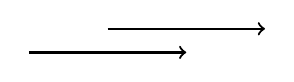
\begin{tikzpicture}=\ReadArrowType]
			\draw[->,style=thick] (0,0) -- (2,0);
			\draw[->,style=thick] (1.0,0.3) -- (3.0,0.3);
		\end{tikzpicture}
		%\vspace{3mm}
		%or (symmetrically)
		%\vspace{3mm}

		%\begin{tikzpicture}=\ReadArrowType]
			%\draw[->,style=thick] (2,0) -- (0,0);
			%\draw[->,style=thick] (3.0,0.3) -- (1.0,0.3);
		%\end{tikzpicture}
		\caption{``Normal'' overlap}
	\end{subfigure}
	\begin{subfigure}[b]{0.3\textwidth}
		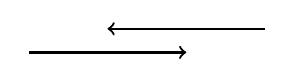
\begin{tikzpicture}=\ReadArrowType]
			\draw[->,style=thick] (0,0) -- (2,0);
			\draw[->,style=thick] (3,0.3) -- (1,0.3);
		\end{tikzpicture}
		\caption{``Innie'' overlap}
	\end{subfigure}
	\begin{subfigure}[b]{0.3\textwidth}
		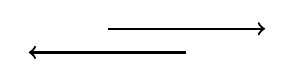
\begin{tikzpicture}=\ReadArrowType]
			\draw[->,style=thick] (2,0) -- (0,0);
			\draw[->,style=thick] (1.0,0.3) -- (3.0,0.3);
		\end{tikzpicture}
		\caption{``Outie'' overlap}
	\end{subfigure}
	\caption{The three types of overlaps.  The innie and outie overlaps are
	reverse-complement overlaps, while the normal overlap is not.  Note:
	with the normal overlap, there is a symmetric case that is not
	considered a distinct type of overlap here.}
	\label{fig:overlap_types}
\end{figure}

%\begin{enumerate}
	%\item ``Normal'' overlap
		%\begin{center}
			%\vspace{-0.5cm}
			%\begin{tikzpicture}[>=\ReadArrowType]
				%\draw[->,style=thick] (0,0) -- (2,0);
				%\draw[->,style=thick] (1.0,0.3) -- (3.0,0.3);
			%\end{tikzpicture}

			%\vspace{3mm}
			%or (symmetrically)
			%\vspace{3mm}

			%\begin{tikzpicture}[>=\ReadArrowType]
				%\draw[->,style=thick] (2,0) -- (0,0);
				%\draw[->,style=thick] (3.0,0.3) -- (1.0,0.3);
			%\end{tikzpicture}
		%\end{center}
	%\vspace{0.5cm}
	%\item ``Innie'' overlap
		%\begin{center}
			%\vspace{-0.5cm}
			%\begin{tikzpicture}[>=\ReadArrowType]
				%\draw[->,style=thick] (0,0) -- (2,0);
				%\draw[->,style=thick] (3,0.3) -- (1,0.3);
		%\end{tikzpicture} \end{center}
	%\vspace{0.5cm}
	%\item ``Outie'' overlap
		%\begin{center}
		%\vspace{-0.5cm}
		%\begin{tikzpicture}[>=\ReadArrowType]
				%\draw[->,style=thick] (2,0) -- (0,0);
				%\draw[->,style=thick] (1.0,0.3) -- (3.0,0.3);
		%\end{tikzpicture} \end{center}
%\end{enumerate}

Overlaps are important because two reads that overlap may come from adjacent
positions on the genome.  Although due to repeats, we cannot be certain that two
overlapping reads actually come from adjacent positions, we {\em can} say for
certain that two reads that do not overlap do not come from adjacent positions
on the genome.  Regardless of this, \Figure{fig:overlap_examples} shows how two
reads that overlap potentially could be combined to form a longer sequence.

\begin{figure}
		%\begin{tikzpicture}
			%\draw (0, 0) node[anchor=left] {Read 1:}	
			%\draw (0, -1) node[anchor=left] {Read 2:}	
			%\draw (0, -2) node[anchor=left] {Possible genome:}
		%\end{tikzpicture}
	\centering
	\begin{subfigure}[t]{0.455\textwidth}
		1: \hspace{0.7mm}{\tt $\rightarrow$ATATAT{GCTGGTTACTT}$\rightarrow$ } \\
		2: \hspace{0.7mm}{\tt \ \ \ \ \ \ $\rightarrow${GCTGGTTACTT}TGATAGATA$\rightarrow$ } \\
		G: {\tt $\rightarrow$ATATATGCTGGTTACTTTGATAGATA$\rightarrow$}
		\caption{A normal overlap between reads (1) and (2) and the
		implied way in which the two reads could be joined together to
		form a longer sequence (G)}
	\end{subfigure}
		\hspace{0.07\textwidth}
	\begin{subfigure}[t]{0.455\textwidth}
		1: \hspace{0.7mm}{\tt $\rightarrow$ATATAT{GCTGGTTACTT}$\rightarrow$ } \\
		2: \hspace{0.7mm}{\tt \ \ \ \ \ \ $\leftarrow${CGACCAATGAA}ACTATCTAT$\leftarrow$ } \\
		G: {\tt $\rightarrow$ATATATGCTGGTTACTTTGATAGATA$\rightarrow$}
		\caption{A reverse-complement overlap between reads (1) and
		(2)--- more specifically, an ``innie'' overlap--- and the
		implied way in which the two reads could be joined together to
		form a longer sequence (G)}
	\end{subfigure}
	\caption{Examples of normal and reverse-complement overlaps}
	\label{fig:overlap_examples}
\end{figure}

\subsection{Computing overlaps}

\subsubsection{Algorithms}

Now that the idea of an exact overlap has been formalized, what we would like to
do is compute all pairwise exact overlaps of minimum length $L$ among the reads
that were provided as input to the assembler.

The naive way to do this is to consider every pair of reads in the input,
including only distinct pairs but also including the special cases of each read
paired with itself, and search for each of the types of overlaps between the two
reads in each pair.  If there are $N$ reads in the input, this algorithm will
need to consider $\frac{N^2}{2} + N$ pairs of reads, and the time spent on each
read pair will depend several factors, including the minimum overlap length and
the read lengths.  But even if we could somehow spend constant time on each read
pair, this algorithm is much too slow because the running time rises quadraticly
with respect to the number of reads.  This is important because there can easily
be millions of reads in the input.

A number of faster algorithms for computing overlaps have been designed.  One of
the easier ones to understand is the \KeyTerm{seed-and-extend} algorithm.  It
works by indexing the reads by short subsequences of a certain length (less than
or equal to than the minimum overlap length) and then only comparing reads that
actually share a subsequence.  Each of these short subsequences is called a
\KeyTerm{seed}.  Two reads may share a seed in either a forward or
reverse-complement manner.  Given two reads that share a seed, the seed can be
extended outwards in both directions in order to find a maximal matched region,
that may be either forward or reverse-complement, between the two reads.  Then,
this maximal matched region is compared against the definition of an overlap.
In particular, it must be at least as long as the minimum overlap length, it
must have least 2 extreme points over the two reads, and it cannot be the prefix
or suffix of both reads if the match does not extend to the opposite end of at
least one of the reads.  If all of these conditions are met and the same overlap
was not already found through another seed in the same two reads, this overlap
is added to the set of overlaps.

The running time of the seed-and-extend algorithm, as described above, is
typically much faster than the naive algorithm, although it is highly dependent
on the data.  For a string of the genome of length $G$ and with a seed length
$k$, there will be at most $G-k+1$ canonical seeds.\footnote{The canonical form
of a DNA sequence and its reverse-complement is the lexicographically lesser of
the two.  Here, we refer canonical form of each seed, because we wish to compare
reads that share a seed in either a forward or reverse-complement manner.}  For
each of these seeds, the reads containing it will be examined exhaustively in a
pairwise manner, which takes quadratic time with respect to the number of reads
sharing that seed.  Since the more densely reads are sampled from the genome,
the more reads will contain each seed,  the running time of the seed-and-extend
algorithm rises quadratically with regards to read density.  In addition, the
number of read pairs the algorithm considers for a specific seed also rises
quadratically with the number of times that seed is repeated in the genome due
to genomic repeats.  Overall, the seed-and-extend algorithm is not ideal and is
still a bottleneck of the entire assembly algorithm, despite the fact that it is
much faster than the naive algorithm (except in degenerate cases, such as a
``genome'' that is entirely a single repeated letter).

\subsubsection{Implementation}

For this project, the seed-and-extend algorithm for computing overlaps was
implemented as the program \ProgramName{compute-overlaps}.  It takes as input a
file that contains a list of reads, as well as a parameter that specifies the
minimum overlap length $L$.  It produces as output (via a data structure
serialized to a file) all exact pairwise overlaps of minimum length $L$ among
reads in the input file, including reverse-complement overlaps and
self-overlaps.  The running time of the algorithm was discussed above.  The
memory usage is linear with respect to the total length of the reads and the
number of overlaps, which likely could be improved.

\begin{comment}
\begin{algorithm}
\caption{{\sc ComputeExactOverlapsNaive}($S$, $L$)}
\begin{algorithmic}
	%\FOR{{\bf each} distinct}
	\STATE b
\end{algorithmic}
\end{algorithm}

\newcommand{\OccVar}{\omega}
%\newcommand{\OccOne}{{\OccVar}_1}
%\newcommand{\OccTwo}{{\OccVar}_2}
\newcommand{\OccOne}{{\tt occ1}}
\newcommand{\OccTwo}{{\tt occ2}}
\newcommand{\SeedVar}{{\tt seed}}
\newcommand{\OccList}{{\tt occurrenceSet}}
\newcommand{\OverlapSet}{{\tt overlapSet}}
\newcommand{\OccMap}{{\tt occurrenceMap}}
\newcommand{\PosOne}{{\tt pos1}}
\newcommand{\PosTwo}{{\tt pos2}}
\newcommand{\Len}{{\tt len}}
\newcommand{\RightExtend}{{\tt rightExtend}}
\newcommand{\LeftExtend}{{\tt leftExtend}}
\newcommand{\ReadSet}{{\tt readSet}}
\newcommand{\minOverlapLen}{{\tt minOverlapLen}}
\newcommand{\readOneBeg}{{\tt read1Begin}}
\newcommand{\readOneEnd}{{\tt read1End}}
\newcommand{\readTwoBeg}{{\tt read2Begin}}
\newcommand{\readTwoEnd}{{\tt read2End}}
\newcommand{\numExtremePoints}{{\tt numExtremePoints}}

\begin{algorithm}
\caption{{\sc ComputeExactOverlapsSeedAndExtend}($\ReadSet$, $\minOverlapLen$)}
\begin{algorithmic}
	%\REQUIRE{$S$ is a list of DNA sequences}
	%\REQUIRE{$L$ is a positive integer that is the minimum overlap length}
	\STATE{Let $k$ be a positive integer less than or equal to
	$\minOverlapLen$.}
	\STATE{Let $\OccMap$ be a hash table that maps DNA sequences to sets of
		$k$-mer occurrences.}
	\STATE{Let $\OverlapSet$ be an empty set of overlaps.}
	\FOR{{\bf each} sequence $s \in \ReadSet$}
		\FOR{{\bf each} canonical $k$-mer $K \in r$}
			\STATE{Add the occurrence of $K$ to $\OccMap[K]$}
		\ENDFOR
	\ENDFOR
	\FOR{{\bf each} $(\SeedVar,\ \OccList) \in \OccMap$}
		\FOR{{\bf each} distinct pair of $k$-mer occurrences $\OccOne,
		\OccTwo \in \OccList$}
			\IF{the read ID of $\OccOne$ is greater than the read ID
			of $\OccTwo$}
				\STATE{Swap $\OccOne$ and $\OccTwo$}
			\ENDIF
			\IF{$\OccOne$ and $\OccTwo$ are both forward or both
			reverse-complement}
				\STATE{${\tt rc} \gets$ {\bf true}}
			\ELSE
				\STATE{${\tt rc} \gets$ {\bf false}}
			\ENDIF
			\STATE{$f \gets$ the read containing $\OccOne$}
			\STATE{$g \gets$ the read containing $\OccTwo$}
			\STATE{$\PosOne \gets$ the position within $f$ of $\OccOne$}
			\STATE{$\PosOne \gets$ the position within $g$ of $\OccTwo$}
			\STATE{$\Len \gets k$}
			\IF{${\tt rc}$}
				\STATE{$g' \gets$ the reverse complement of $g$}
				\STATE{${\tt \LeftExtend} \gets$ the number of
				additional bp to the left of the seed that
				match, comparing $f$ with $g'$}
				\STATE{${\tt \RightExtend} \gets$ the number of
				additional bp to the right of the seed that
				match, comparing $f$ with $g'$}
				\STATE{$\PosTwo \gets \PosTwo - {\tt
				\RightExtend}$}
			\ELSE
				\STATE{${\tt \LeftExtend} \gets$ the number of
				additional bp to the left of the seed that
				match, comparing $f$ with $g$}
				\STATE{${\tt \RightExtend} \gets$ the number of
				additional bp to the right of the seed that
				match, comparing $f$ with $g$}
				\STATE{$\PosTwo \gets \PosTwo - {\tt \LeftExtend}$}
			\ENDIF
			\STATE{$\PosOne \gets \PosOne - {\tt \LeftExtend}$}
			\STATE{$\Len \gets \Len + {\tt \LeftExtend} + {\tt \RightExtend}$}
			\IF{$\Len < \minOverlapLen$} 
				\STATE{\bf continue}
			\ENDIF
			\STATE{$\readOneBeg \gets \PosOne$}
			\STATE{$\readOneEnd \gets \PosOne + \Len - 1$}
			\STATE{$\readTwoBeg \gets \PosTwo$}
			\STATE{$\readTwoEnd \gets \PosTwo + \Len - 1$}
			\STATE{$\numExtremePoints \gets 0$}
			\IF{$\readOneBeg = 0$}
				\STATE{$\numExtremePoints \gets \numExtremePoints + 1$}
			\ENDIF
			\IF{$\readOneEnd = {\sc Length}(f) - 1$}
				\STATE{$\numExtremePoints \gets \numExtremePoints + 1$}
			\ENDIF
			\IF{$\readTwoBeg = 0$}
				\STATE{$\numExtremePoints \gets \numExtremePoints + 1$}
			\ENDIF
			\IF{$\readTwoEnd = {\sc Length}(g) - 1$}
				\STATE{$\numExtremePoints \gets \numExtremePoints + 1$}
			\ENDIF


			%\STATE{Maximally extend the occurrence of $\SeedVar$ at
			%$\OccOne$ and $\OccTwo$ outwards in both directions}
			%\STATE{${\tt pos1} \gets$ the beginning of the maximally
			%matched region on the read containing $\OccOne$}
			%\STATE{${\tt pos2} \gets$ the beginning of the maximally
			%matched region on the read containing $\OccTwo$}
			%\STATE{${\tt plen} \gets$ the length of the maximall
			%matched region on the read containing $\OccTwo$}
		\ENDFOR
	\ENDFOR
\end{algorithmic}
\end{algorithm}
\end{comment}


\section{Building the fragment string assembly graph}

\subsection{Overview}

After overlaps have been computed from the reads, the next step is to construct
a graph that models how the reads can be assembled together when the overlaps
are used as evidence.  To do this, define a graph where each vertex corresponds
to a read and each edge corresponds to an overlap.  Two vertices are connected
by an edge if and only if the corresponding reads share an overlap.  In
addition, each edge is labeled with an appropriate DNA sequence, the details of
which will be explained later.

It needs to be decided whether each edge will be directed, undirected, or
something else.  To decide this, we need to consider exactly what we want each
edge to actually represent.  Consider three reads $f$, $g$, and $h$, that
overlap as follows:

\begin{center}
	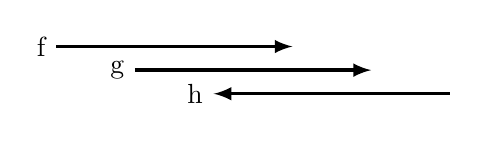
\begin{tikzpicture}[>=\ReadArrowType]
		\draw[->,style=very thick] (0,   0.6) node[anchor=east] {f} -- (3.0, 0.6);
		\draw[->,style=very thick] (1.0, 0.3) node[anchor=east] {g} -- (4.0, 0.3);
		\draw[<-,style=very thick] (2.0, 0.0) node[anchor=east] {h} -- (5.0, 0.0);
	\end{tikzpicture}
\end{center}

There are 3 overlaps so there will be 3 edges--- one between $f$ and $g$, one
between $g$ and $h$, and one between $f$ and $h$.  As shown, the reads can be
assembled together consistently when used in the order $f,\ g,\ h$; therefore, it
must be possible to walk $f \to g \to h$ in the graph to model this assembly.
In addition, these reads could actually spell out the reverse-complement
sequence instead:

\begin{center}
	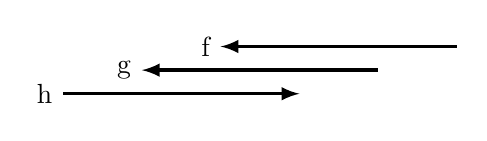
\begin{tikzpicture}[>=\ReadArrowType]
		\draw[->,style=very thick] (0,   0.0) node[anchor=east] {h} -- (3.0, 0.0);
		\draw[<-,style=very thick] (1.0, 0.3) node[anchor=east] {g} -- (4.0, 0.3);
		\draw[<-,style=very thick] (2.0, 0.6) node[anchor=east] {f} -- (5.0, 0.6);
	\end{tikzpicture}
\end{center}

Therefore, the walk $h \to g \to f$ must be allowed.  Furthermore, read $f$
directly overlaps with read $h$, so it must also be possible to walk directly $f
\to h$ or $h \to f$.


We might consider a directed graph, but this does not work because the graph
does not allow the reverse-complement walks such as $h \to g \to f$:

\begin{center}
	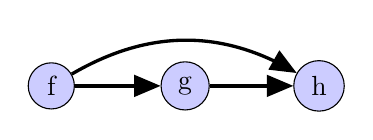
\begin{tikzpicture}[>=triangle 45]
		\tikzstyle{every node} = [circle,fill=blue!20,draw=black];
		\node (f) at (0, 0) {f};
		\node (g) at (1.7, 0) {g};
		\node (h) at (3.4, 0) {h};
		\draw[->,style=very thick] (f) edge (g);
		\draw[->,style=very thick] (g) edge (h);
		\draw[->,style=very thick,bend left] (f) edge (h);
	\end{tikzpicture}
\end{center}

Similarly, we might consider an undirected graph, but this does not work because
the graph fails to disallow walks such as $g \to h \to f$ that correspond to
assemblies that are not supported by the underlying reads.

\begin{center}
	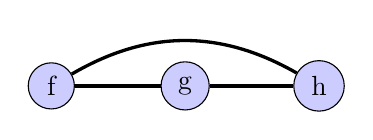
\begin{tikzpicture}[>=triangle 45]
		\tikzstyle{every node} = [circle,fill=blue!20,draw=black];
		\node (f) at (0, 0) {f};
		\node (g) at (1.7, 0) {g};
		\node (h) at (3.4, 0) {h};
		\draw[-,style=very thick] (f) edge (g);
		\draw[-,style=very thick] (g) edge (h);
		\draw[-,style=very thick,bend left] (f) edge (h);
	\end{tikzpicture}
\end{center}

The fundamental problem with using the directed graph is that at this stage in
the assembly, we don't know in absolute terms which strand a given read is from.
Given two reads that overlap, we can say if they are probably from the same
strand or probably from opposite strands, but we cannot say {\em in absolute
terms} which strand a given read is from.  Therefore, we must allow each read to
be used in either the forward or reverse-complement direction.  This implies
that it needs to be possible to traverse each edge in either direction, since
flipping the order of the reads in an overlap, in effect, implies that they are
reverse-complemented.  The undirected graph satisfies these requirements, but it
fails in another way: it has no guarantee that a given read is used in a
consistent way at a location within any single assembly.

The solution to all these problems is to use a new type of graph called a
\KeyTerm{bidirected graph}:
\begin{center}
	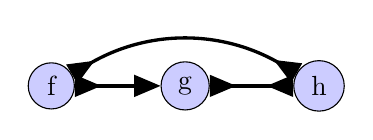
\begin{tikzpicture}[>=triangle 45]
		\tikzstyle{every node} = [circle,fill=blue!20,draw=black];
		\node (f) at (0, 0) {f};
		\node (g) at (1.7, 0) {g};
		\node (h) at (3.4, 0) {h};
		\draw[>->,style=very thick] (f) edge (g);
		\draw[>-<,style=very thick] (g) edge (h);
		\draw[>-<,style=very thick,bend left] (f) edge (h);
	\end{tikzpicture}
\end{center}

\subsection{Bidirected graphs}

A \KeyTerm{bidirected graph} is a graph where a directed head is attached to both
ends of each edge.

There are 3 (or 4, ignoring symmetry) types of \KeyTerm{bidirected edges}.  They
follow directly from the different types of overlaps (see
\Figure{fig:overlap_mapping}).

\begin{figure}
	\begin{center}
		\begin{tabular}{p{1cm}cccc}
			{\footnotesize Overlap} &
			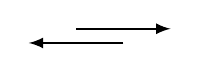
\begin{tikzpicture}[scale=0.6,>=\ReadArrowType]
					\draw[->,style=thick] (2,0) -- (0,0);
					\draw[->,style=thick] (1,0.3) -- (3,0.3);
			\end{tikzpicture}
			&
			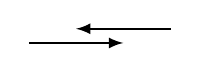
\begin{tikzpicture}[scale=0.6,>=\ReadArrowType]
					\draw[->,style=thick] (0,0) -- (2,0);
					\draw[->,style=thick] (3,0.3) -- (1,0.3);
			\end{tikzpicture}
			&
			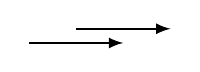
\begin{tikzpicture}[scale=0.6,>=\ReadArrowType]
					\draw[->,style=thick] (0,0) -- (2,0);
					\draw[->,style=thick] (1,0.3) -- (3,0.3);
			\end{tikzpicture}
			&
			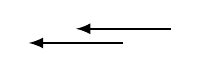
\begin{tikzpicture}[scale=0.6,>=\ReadArrowType]
					\draw[->,style=thick] (2,0) -- (0,0);
					\draw[->,style=thick] (3,0.3) -- (1,0.3);
			\end{tikzpicture}
			\\
			&$\downarrow$ & $\downarrow$& $\downarrow$& $\downarrow$ \\
			{\footnotesize Bidirected edge} &
			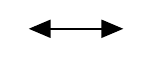
\begin{tikzpicture}[scale=0.6,>=triangle 45]
					\draw[<->,style=thick] (0,0) -- (2,0);
			\end{tikzpicture}
			&
			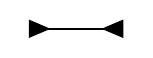
\begin{tikzpicture}[scale=0.6,>=triangle 45]
					\draw[>-<,style=thick] (0,0) -- (2,0);
			\end{tikzpicture}
			&
			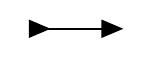
\begin{tikzpicture}[scale=0.6,>=triangle 45]
					\draw[>->,style=thick] (0,0) -- (2,0);
			\end{tikzpicture}
			&
			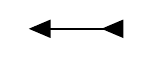
\begin{tikzpicture}[scale=0.6,>=triangle 45]
					\draw[<-<,style=thick] (0,0) -- (2,0);
			\end{tikzpicture}
		\end{tabular}
	\end{center}
	\caption{Mapping from the types of overlaps to the types of bidirected edges.}
	\label{fig:overlap_mapping}
\end{figure}

A \KeyTerm{walk in a bidirected graph} $G$ is a continuous sequence of edges in
$G$ such that if any vertex $v$ is entered through a head inwards, it is exited
through a head outwards (unless it is the end of the path), and vice versa.  An
equivalent formulation is that if we consider a possible walk in a bidirected
graph, such as the possible walk $1 \to 2 \to 3 \to 4$ in the graph shown in
\Figure{fig:bidiwalk_example}, in order to check whether the walk is valid or
not, we must consider every vertex in the possible walk except for the very
first and last vertices.  For each such vertex, we need to verify that each time
that vertex is passed through as part of a walk, the arrow heads adjacent to
that vertex that are used in the relevant part of the walk are pointed in the
same direction {\em relative to the walk}. If there are no such pairs of heads
that point towards each other or point away from each other, the walk is valid.
The red circles in \Figure{fig:bidiwalk_example} show the two pairs of heads
that need to be checked for the possible walk $1 \to 2 \to 3 \to 4$.  

Note that this definition is symmetric, which implies that the reverse of a walk
in a bidirected graph is also a valid walk (e.g. the walk $4 \to 3 \to 2 \to 1$
in \Figure{fig:bidiwalk_example}).  A bidirected edge may be traversed in either
direction, possibly even during the same walk.

\begin{figure}
	\begin{center} {\small
		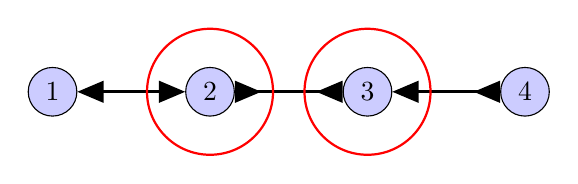
\begin{tikzpicture}[>=triangle 45]
			\tikzstyle{every node} = [circle,fill=blue!20,draw=black];
			\node (1) at (0.00, 0) {1};
			\node (2) at (2.00, 0) {2};
			\node (3) at (4.00, 0) {3};
			\node (4) at (6.00, 0) {4};
			\draw[<->,very thick] (1) edge (2);
			\draw[>-<,very thick] (2) edge (3);
			\draw[<-<,very thick] (3) edge (4);
			\draw[color=red,thick] (2.00, 0) circle (0.8);
			\draw[color=red,thick] (4.00, 0) circle (0.8);
		\end{tikzpicture}
	} \end{center}
	\caption{$1 \to 2 \to 3 \to 4$ and $4 \to 3 \to 2 \to 1$ are both valid walks in
	the bidirected graph below.  (Check circled pairs of heads.)}
	\label{fig:bidiwalk_example}
\end{figure}

\section{Removing contained reads}


\section*{Acknowledgments}

Acknowledgements

\bibliographystyle{plain}
\bibliography{refs}

\end{document}
